\documentclass[compress]{beamer}
\setbeamercovered{transparent}
\usepackage[utf8]{inputenc}


\usepackage{multirow,rotating}
\usepackage{color}
\usepackage{hyperref}
\usepackage{tikz-cd}
\usepackage{array}
\usepackage{siunitx}
\usepackage{mathtools,nccmath}%
\usepackage{etoolbox, xparse}
\usepackage{adjustbox}
\usetheme{CambridgeUS}
\usecolortheme{dolphin}
\usepackage{graphics}
\usepackage{media9}
\usepackage{graphicx}

% set colors
\definecolor{myNewColor0}{RGB}{33, 39, 39}   % dark gray
\definecolor{myNewColorA}{RGB}{226, 220,200}   % yellow 
%\definecolor{myNewColorA}{RGB}{235, 231, 217}
\definecolor{myNewColorB}{RGB}{241, 241,241} % white
\definecolor{myNewColorC}{RGB}{60, 70,70} % dark green
\setbeamercolor*{palette primary}{bg=myNewColorA, fg = myNewColor0}
\setbeamercolor*{palette secondary}{bg=myNewColorA, fg = myNewColor0}
\setbeamercolor*{palette tertiary}{bg=myNewColorA, fg = myNewColor0}
\setbeamercolor*{title}{bg=myNewColorA, fg = myNewColor0}
\setbeamercolor*{titlelike}{bg=myNewColor0, fg=myNewColorB}
\setbeamercolor*{item}{fg=myNewColorA}
\setbeamercolor*{caption name}{fg=myNewColor0}
\setbeamercolor*{block title}{fg=myNewColor0, bg = myNewColorA}
\setbeamercolor*{block body}{bg = myNewColorB, fg = myNewColor0}

\usefonttheme{professionalfonts}
\setbeamercolor*{subsection in head/foot}{bg=myNewColorB,fg=black}
\setbeamercolor{page number in head/foot}{fg=myNewColor0}
\setbeamercolor{background canvas}{bg=myNewColor0}
\setbeamercolor{frametitle}{bg=myNewColorC, fg = myNewColorA}
\setbeamercolor{normal text}{fg=myNewColorA}
%\setbeamercovered{transparent}
\setbeamercovered{invisible}


% no shadow
\setbeamertemplate{title page}[default][colsep=-4bp,rounded=true]
\setbeamertemplate{blocks}[rounded][shadow=false]
\setbeamertemplate{itemize items}[circle]


\setbeamertemplate{headline}{%
  \begin{beamercolorbox}[colsep=1.5pt]{upper separation line head}
  \end{beamercolorbox}
  \begin{beamercolorbox}{section in head/foot}
    \vskip-0.2pt\insertnavigation{\paperwidth}\vskip2pt
  \end{beamercolorbox}%
  \begin{beamercolorbox}[colsep=1.5pt]{lower separation line head}
  \end{beamercolorbox}
}
\makeatother

\setbeamertemplate{bibliography item}[text]

\setbeamertemplate{frametitle}{%
    \nointerlineskip%
    \begin{beamercolorbox}[wd=\paperwidth,ht=25pt,dp = 1pt]{frametitle}
        \hspace*{10pt}\insertframetitle\vskip5pt
    \end{beamercolorbox}%
}

% Author, title, note
\setbeamercolor{bibliography entry author}{fg=myNewColorA}
\setbeamercolor{bibliography entry title}{fg=myNewColorA}
\setbeamercolor{bibliography entry note}{fg=myNewColorA}
\usepackage{hyperref}

\titlegraphic{%
%
\includegraphics[width=2cm]{UvA.png}
%
\includegraphics[width=2cm]{CCI.png}

\includegraphics[width=2.5cm]{MNS.png}
%
\includegraphics[width=2cm]{PCS.png}
}
% set font size
\setbeamerfont{title}{size=\Large}
\setbeamerfont{subtitle}{size=\large}
\setbeamerfont{author}{size=\large}
\setbeamerfont{date}{size=\small}
\setbeamerfont{institute}{size=\large}
\setbeamerfont{block title}{size=\normalsize}
\setbeamerfont{block body}{size=\footnotesize}
%\setbeamerfont{itemize/enumerate body}{family=\sffamily, size={\fontsize{18}{18}}}
\setbeamerfont{itemize/enumerate subbody}{size={\scriptsize}}
\title[Title shown in the bar]{The title of this presentation} %title
\subtitle{} % subtitle
\author[Your email]{Your name}
\institute[Informatics Institute]{University of Amsterdam}
\date[{\today}]\today

%------------------------------------------------------------
%beginning of each section and highlights the current section:
%\AtBeginSection[]
%{
%  \begin{frame}
%    \frametitle{Contents}
%    \tableofcontents[currentsection]
%  \end{frame}
%}
\AtBeginSection[]{
  \begin{frame}
  \vfill
  \centering
  \begin{beamercolorbox}[sep=8pt,center,shadow=false,rounded=true]{title}
    \usebeamerfont{title}\insertsectionhead\par%
  \end{beamercolorbox}
  \vfill
  \end{frame}
}
% Citations can be put into the .bibexample.bib file
\usepackage[style=ieee,citetracker=true, backend=biber]{biblatex}
\addbibresource{bibexample.bib}


% ------Contents below------
\begin{document}

% The next statement creates the title page.

\frame[plain]{\titlepage} % without bottom bar
%\begingroup 			  % with bottom bar
%    \setbeamertemplate{headline}{}
%    \begin{frame}
%        \titlepage
%    \end{frame}
%\endgroup

%% If the content is not that much, can delete the table of content page
% \begin{frame}
% \frametitle{Outline}
% \tableofcontents
% \end{frame}

%------------------------------------------------------------
%\section*{Section1} % do not show section page
\section{Section1} % show section page

\setbeamertemplate{background}
{
    
\includegraphics[width=\paperwidth,height=\paperheight]{UvA-bg.png}
}

\subsection{Section1.1}
\begin{frame}{Background} 
    \begin{itemize} %[<+->] % More beamer overlay Beamer Overlay Specifications can be found in "https://www.overleaf.com/learn/latex/Beamer_Presentations%3A_A_Tutorial_for_Beginners_(Part_4)%E2%80%94Overlay_Specifications"
        \item Point1
            \begin{center}
                \begin{minipage}{10.3cm}
                \begin{block}{Block Title}
                    Content of the block.
                \end{block}
                \end{minipage}
            \end{center}
        \item[] % add a space line
        \item Point2
            \begin{itemize}
                \item item1
                \item item2
                \item item3
            \end{itemize}
        \item Point3
    \end{itemize}
\end{frame}

\subsection{Section1.2}
\begin{frame}{Preliminaries}
    \begin{itemize}
        \item<1-> Preliminary a
        \item<1-> Preliminary a'
        \item<2-> Preliminary b
    \end{itemize}
\end{frame}

\section{Section2}
\subsection{Model}
\begin{frame}{Name of the model\cite{zhou2022costly}}
%\begin{frame}{\href{you can add your github link}{Sustainable Incentive Design~\cite{or add citations}}}
    \begin{columns}[c]
    % create the column: images-left, text-right
    
    % images
        \begin{column}{.5\textwidth}
            \centering
            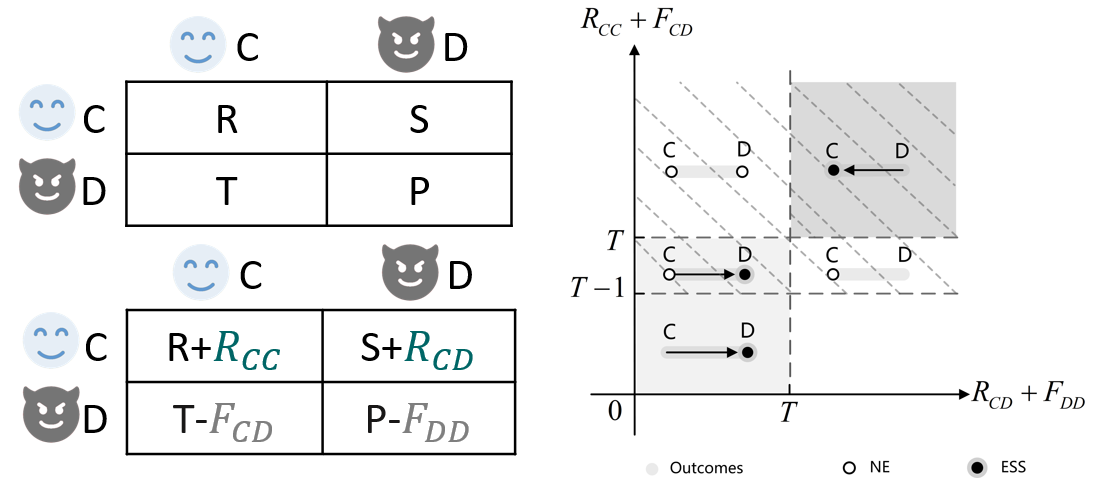
\includegraphics[width=\textwidth]{ProperIncentAnaModel.png}\\[0.5cm]
            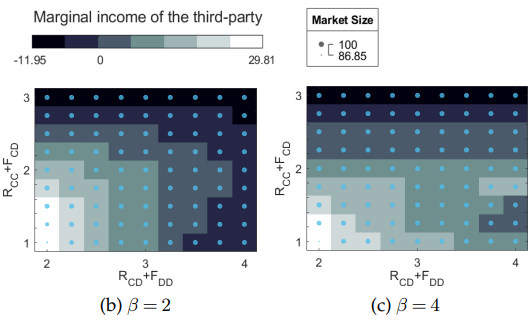
\includegraphics[width=0.9\textwidth]{ProperIncentExpResult.png}\\[0.5cm]
        \end{column}
    
    % texts
        \begin{column}{.5\textwidth}
            \raggedright
            \begin{minipage}{5.8cm}
                \begin{block}{Concept1}
                    babababbababababa
                \end{block}
                \begin{block}{Concept2}
                    \textbf{LALALALALALA}:\\
                    \begin{itemize}
                        \item LA1
                        \item LA2
                        \begin{itemize}
                        	\item LA11
                        	\item LA12
                        \end{itemize}
                    \end{itemize}
                \end{block}
            \end{minipage}
        \end{column}
    \end{columns}
\end{frame}

\begin{frame}
	\printbibliography
\end{frame}

\begin{frame}
    \titlepage
\end{frame}

\end{document}



